\section{Introduction}
\label{sec:introduction}

% ── Instructions ─────────────────────────────────────────────────────────
% Structure: hook → problem → gap → contribution → paper outline (1 paragraph each).
% End with a bullet list of contributions.
% ─────────────────────────────────────────────────────────────────────────

Autonomous mobile robots operating in indoor environments must maintain an
accurate global pose estimate to navigate safely, revisit places reliably, and
build maps that remain useful over long deployments. At a high level, SLAM can
be interpreted as a probabilistic estimation problem in which the robot seeks
to infer its trajectory and the map from a stream of noisy controls and sensor
measurements. Classical Bayesian filtering formulations, including
Kalman-filter variants and particle-filter methods such as FastSLAM,
update this belief recursively as new observations arrive
~\cite{montemerlo2003fastslam,sunderhauf2007ukfslam}. This recursive structure
makes them attractive for online operation and for tightly coupled multi-sensor
fusion, where camera, LiDAR, and IMU measurements must be integrated at
different rates within a common state-estimation framework~\cite{zhu2024survey}.
At the same time, filtering approaches commit to local updates as data arrive,
which makes it less natural to incorporate long-range dependencies, delayed
loop closures, and global consistency corrections than in full smoothing or
factor-graph formulations.

\begin{figure}[t]
      \centering
      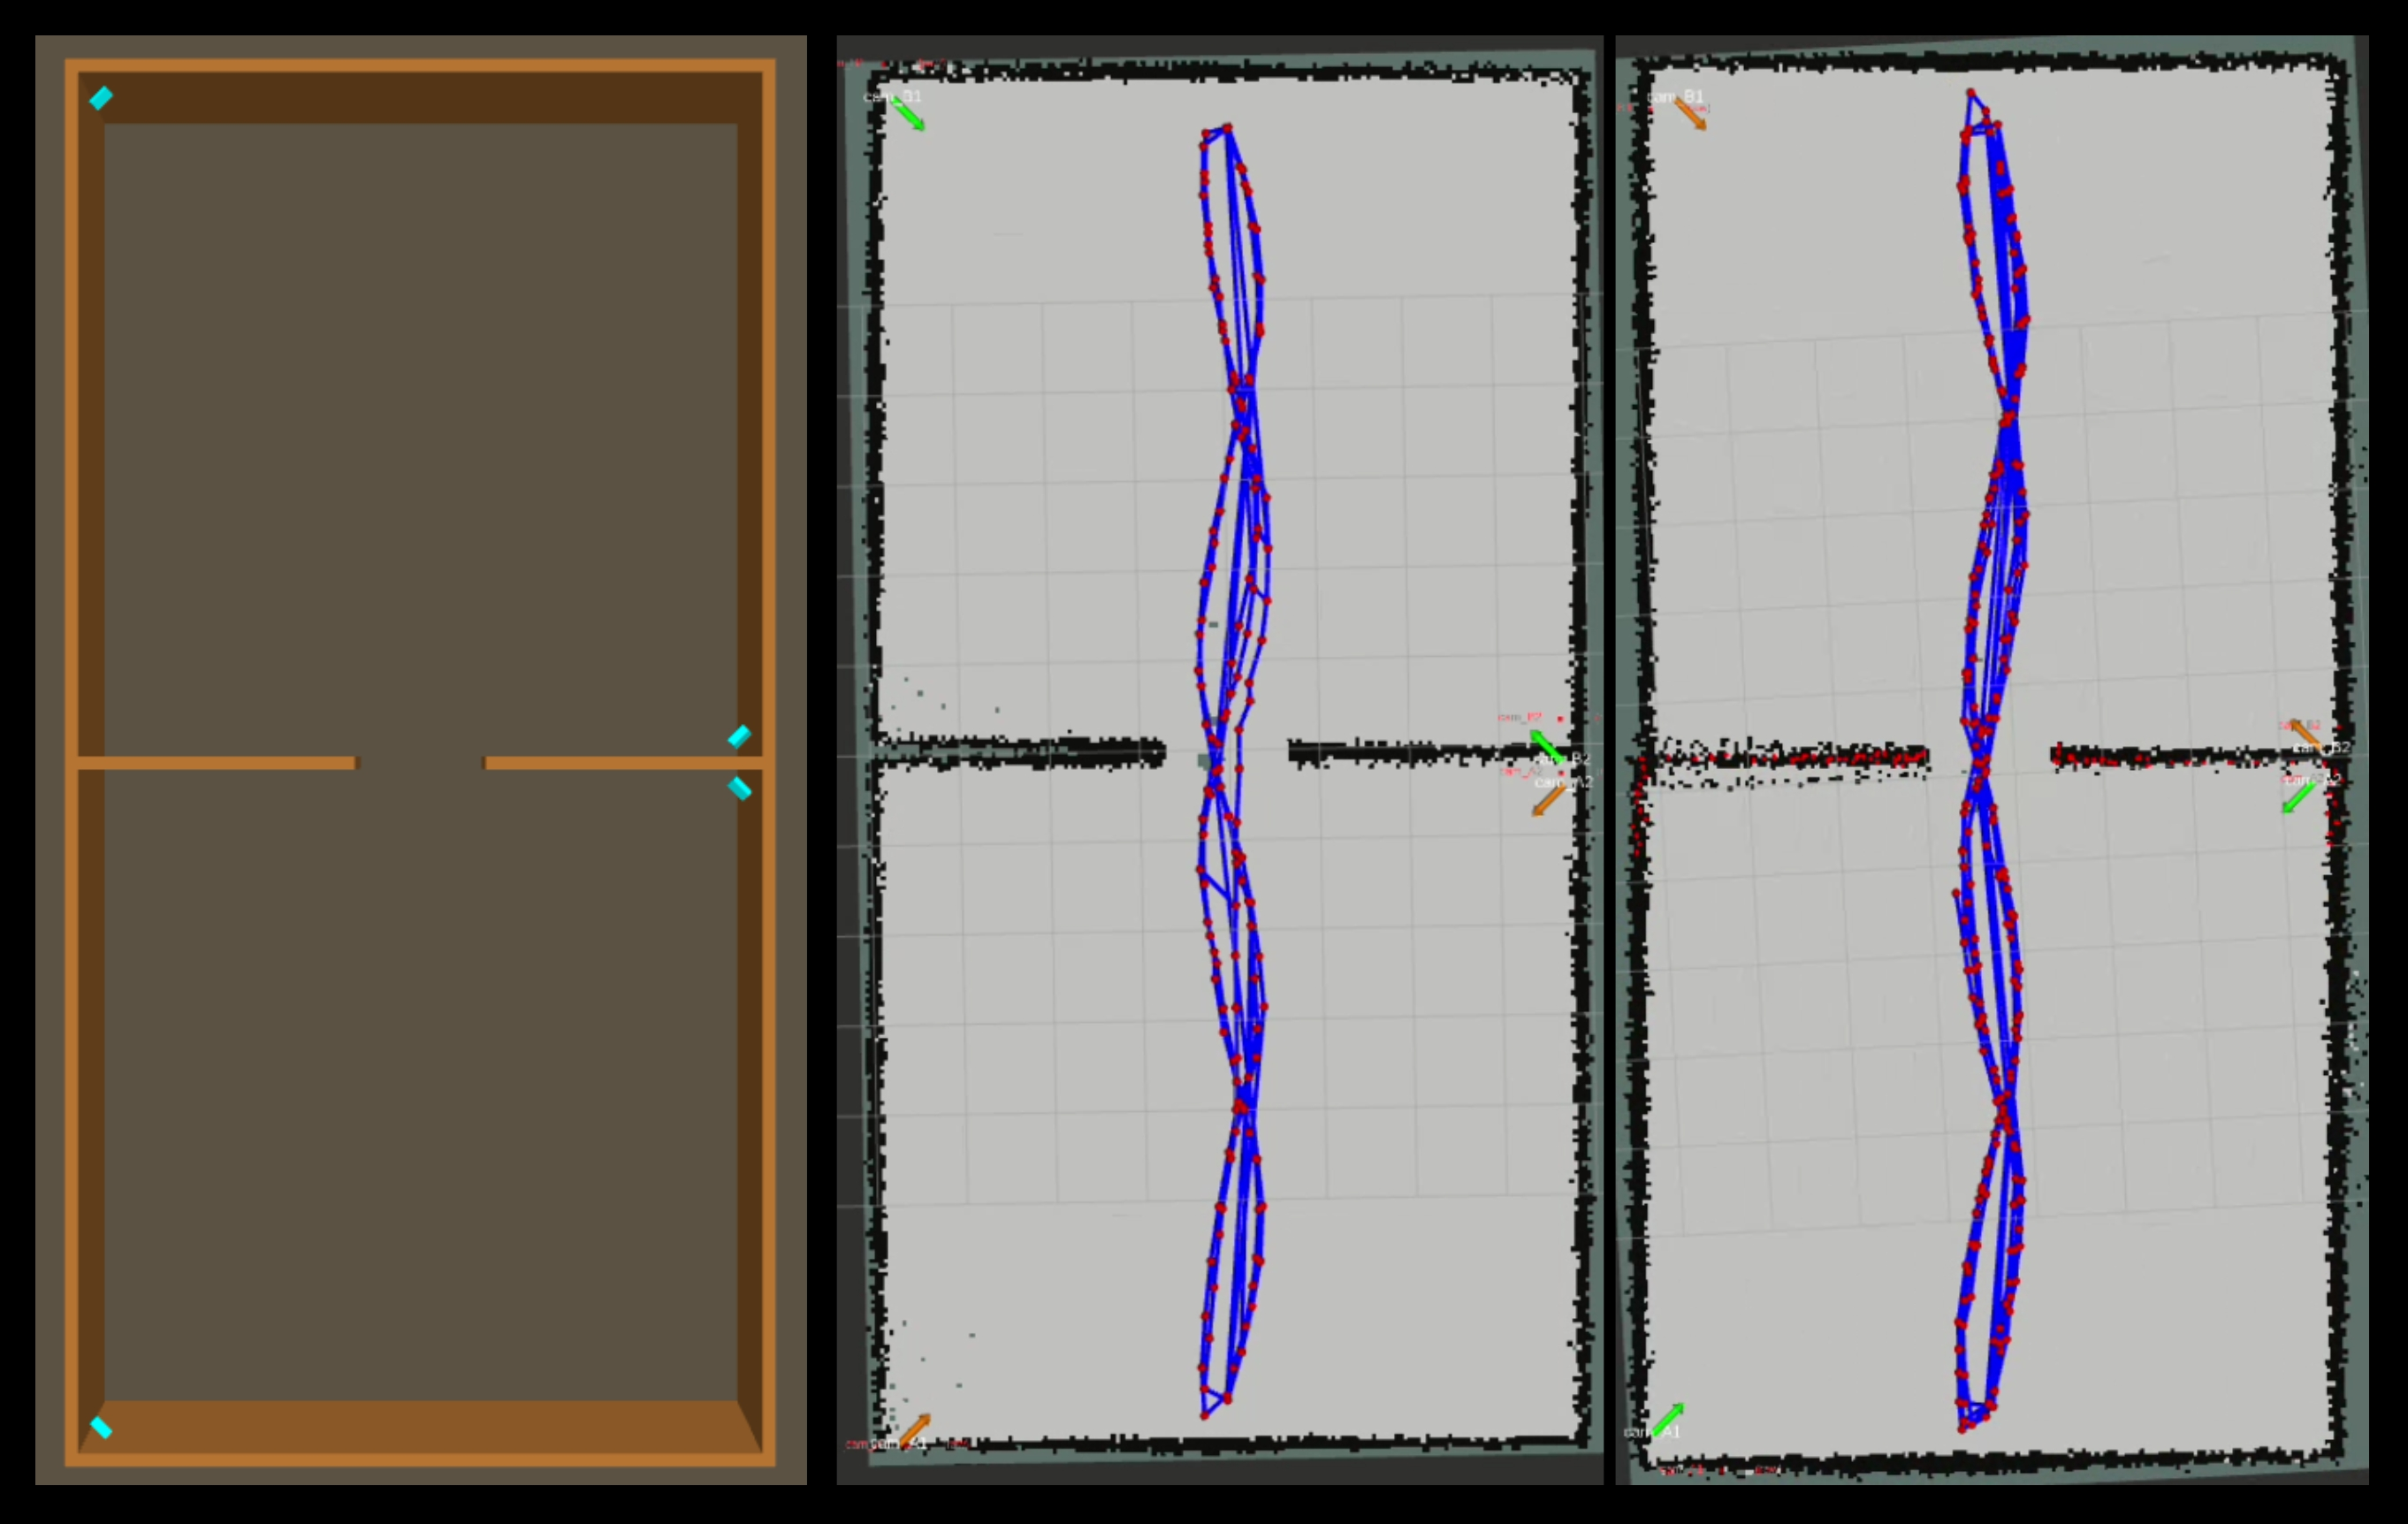
\includegraphics[width=\linewidth]{figures/overview.jpg}
      \caption{Qualitative overview of the 2-room scenario.
               \textbf{Left:} Gazebo environment.
               \textbf{Middle:} LiDAR-only SLAM --- a camera marker is misregistered into the neighbouring room.
               \textbf{Right:} Proposed method --- camera nodes remain in the correct room corners.}
      \label{fig:qualitative_overview}
\end{figure}

Graph-based SLAM addresses these limitations by representing robot poses and
map variables as nodes in a sparse factor graph and encoding odometry,
scan-matching, and loop-closure measurements as constraints between them.
Inference then becomes a nonlinear optimisation problem over the full graph,
which enables robust global refinement and has made graph-based methods a
dominant formulation for modern SLAM back-ends~\cite{grisetti2010tutorial,sunderhauf2012robust}.
This is also the setting adopted by the 2D LiDAR SLAM backend used in
this work~\cite{macenski2021slam}. However,
for 2D LiDAR-based systems operating in large, repetitive, or featureless
environments such as corridors, open halls, or sparsely structured rooms,
drift can remain significant even after loop closures because local scan
geometry is often insufficiently distinctive and the available constraints are
too weak to anchor the map globally.

One way to supply stronger global information is to exploit an infrastructure
camera network. Fixed ceiling- or wall-mounted cameras observe the robot from
stable viewpoints that are decoupled from the robot's own motion and can
therefore provide complementary constraints to onboard LiDAR. Recent work such
as YOWO~\cite{yang2025yowo} has shown that jointly mapping an indoor scene and
registering ceiling-mounted cameras can improve both scene reconstruction and
camera registration. That observation is directly relevant here: when cameras
are registered only after a SLAM map has already been created, any residual map
drift is inherited by the camera poses and later reused as a biased reference.
At the same time, YOWO focuses on RGB-D scene capture and scene-layout
registration, whereas our target problem is 2D LiDAR SLAM supported by
sparse visual anchor constraints from fixed infrastructure cameras during
mapping.

This paper explores that gap by augmenting a 2D LiDAR pose graph with
camera-derived constraints so that infrastructure observations contribute to
global consistency during optimisation rather than only after a separate manual
registration stage.

Figure~\ref{fig:qualitative_overview} illustrates this contrast: without
camera constraints the pose-graph drifts and misregisters a camera marker
into the wrong room, whereas the proposed augmentation keeps all camera nodes
consistent with their correct room corners after optimisation.

We address this gap by contributing:

\begin{itemize}
    \item A constraint formulation that injects a camera-to-robot relative
          observation into a Ceres~\cite{ceres-solver} pose graph whenever the
          robot is visually detected, with per-axis covariance weighting.
    \item A camera-based robot pose estimation pipeline that injects visual
          anchor constraints into the pose graph of the LiDAR SLAM backend
          without replacing the underlying 2D LiDAR SLAM pipeline.
    \item An experimental evaluation in simulated 2-room, 5-room, and 10-room
          ring environments demonstrating measurable reduction in absolute
          trajectory error compared to a LiDAR-only baseline.
\end{itemize}

The remainder of this paper is organised as follows.
Section~\ref{sec:related_work} reviews related work.
Section~\ref{sec:methodology} describes the constraint formulation and
system architecture.
Section~\ref{sec:experiments} details the experimental setup.
Section~\ref{sec:results} presents and discusses results.
Section~\ref{sec:conclusion} concludes.
